\chapter{Active Vision and perception for human robot interaction}
Nel mondo reale, gli agenti sono forzati a prendere delle decisioni sulla base
decisioni informazioni incomplete, anche se gli agenti possono acquisire
informazioni raramente ottengono lo stato corretto del mondo.

L'idea per risolvere questo problema è quella di rappresentare esplicitamente
l'incertezza attraverso il calcolo della probabilità.

Possiamo distinguere due obiettivi principali:
\begin{itemize}
    \item \textbf{Percezione attiva}: l'agente deve decidere quali azioni
          intraprendere per ottenere informazioni utili per il compito corrente.
    \item \textbf{Controllo attivo}: l'agente deve decidere quali azioni
          intraprendere per ottenere il miglior risultato possibile.
\end{itemize}
\section{Markov Localization}
\textbf{Markov Localization} è un algoritmo di localizzazione basato su una mappa
dell'ambiente e su un modello di movimento e di osservazione.

L'idea è quella di rappresentare la posizione dell'agente come una distribuzione
di probabilità sullo spazio delle posizioni possibili.

Inizialmente, se un agente non sa dove si trova nell'ambiente, è ragionevole
pensare che la sua conoscenza a priori sia uniforme ($\overline{bel}(x_t)$).
A questo punto viene eseguita una lettura dei sensori e viene calcolata la
nuova distribuzione usando il teorema di Bayes:
\begin{equation}
    bel(x_t) = \eta \cdot p(z_t|x_t) \overline{bel}(x_{t-1})
\end{equation}
dove $\eta$ è il fattore di normalizzazione, mentre $p(z_t|x_t)$ è la probabilità
di osservare $z_t$ dato che l'agente si trova in $x_t$.

L'agente non è statico ma si muove, il che introduce del rumore nella stima.
Possiamo quindi calcolare lo stato successivo come:
\begin{equation}
    bel(x_t) = \int p(x_t|x_{t-1},u_t) bel(x_{t-1}) dx_{t-1}
\end{equation}

Quanto descritto fino a questo momento può essere rappresentato graficamente nel
seguente modo:
\begin{figure}[!ht]
    \centering
    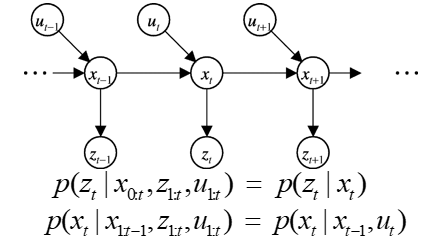
\includegraphics[scale=0.5]{./img/ActiveVision/markov_localization.png}
    \caption{Markov Localization}
    \label{fig:markov_localization}
\end{figure}
Dobbiamo considerare che questo viene fatto sulla base delle seguenti assunzioni:
\begin{itemize}
    \item Il mondo è statico.
    \item Non ci sono errori di approssimazione.
    \item È indipendente dal rumore.
\end{itemize}
La formula di Bayes può essere aggiornata in modo ricorsivo se consideriamo l'assunzione
di Markov, ovvero che $z_n$ è indipendente da $z_1, \dots, z_{n-1}$ dato $x$:
\begin{equation}
    P(x | z_1, \dots, z_n) = \eta_{1 \dots n} \prod_{i=1}^{n} P(z_i | x) P(x)
\end{equation}
\section{Bayesian Filtering}
\textbf{Bayesian Filtering} è un algoritmo di stima che permette di stimare lo stato
di un sistema dinamico a partire da una serie di osservazioni.

In particolare, dati:
\begin{itemize}
    \item Uno stream di osservazioni $z_1, z_2, \dots, z_n$ e di comandi $u_1,
              u_2, \dots, u_n$, denotato con $d_t = \{u_1, z_1, \dots, u_t, z_t\}$.
    \item Una percezione di un sensore $P(z|x)$.
    \item Un modello di transizione di stato $P(x|x',u)$.
    \item Una conoscenza a priori $P(x)$ dello stato.
\end{itemize}
vogliamo stimare lo stato $X$ di un sistema dinamico la cui probabilità a posteriori
$bel(x_t)$ è data da:
\begin{equation}
    bel(x_t) = P(x_t | u_1, z_1, \dots, u_t, z_t) = \dots = 
    \eta P(z_t|x_t) \int P(x_t|u_t, x_{t - 1})bel(x_{t - 1})dx_{t - 1}
\end{equation} 
\section{Utility Optimization}
Vogliamo ora capire come un agente possa prendere delle decisioni in un ambiente 
che lo portino a massimizzare una funzione di ricompense. Solitamente si valutano 
delle funzioni che mi dicono quanto è buono per un agente trovarsi in quello stato.

Dobbiamo distinguere due possibilità:
\begin{itemize}
    \item \textbf{Probabilistic Planning}: l'agente deve prendere decisioni
          conoscendo l'ambiente e la sua dinamica.
    \item \textbf{Reinforcement Learning}: l'agente deve prendere decisioni senza
          conoscere l'ambiente, ma imparando dall'esperienza.
\end{itemize}
I comportamenti e le strategie di azioni diventano delle \textbf{policy} $\pi$,
le quali definisco che azione bisogna intraprendere in ogni stato.

Una reward è rappresentata da uno scalare, indicato con $r_t$ e indica quanto 
un agente si sta comportando nell'istante $t$. Il suo obiettivo è sempre quello 
di massimizzare la reward totale.

Un esempio di una funzione che si vuole massimizzare può essere la seguente:
\begin{equation}
    R_t = \sum_{i=0}^{\infty} \gamma^i r_{t + i}
\end{equation}
dove $\gamma$ è un fattore di sconto che indica quanto è importante la reward
nel futuro rispetto a quella attuale. Nella pratica, questo valore serve per 
evitare che la somma delle reward sia infinita.

Dato che stiamo lavorando con l'incertezza, introduciamo la seguente notazione 
per indicare il valore atteso:
\begin{equation}
    \mathcal{R}_t = \mathbb{E}[R_t] = \mathbb{E}\left[\sum_{i=0}^{\infty} 
    \gamma^i r_{t + i}\right] = \sum_{i = 0}^{\infty} \mathbb{E}[\gamma^i r_{t + i}]
\end{equation}
Questo ci permette di scrivere la funzione in un formato più compatto:
\begin{equation}
    \mathcal{R}_t = \mathbb{E}[r_t] + \gamma \mathcal{R}_{t + 1} 
\end{equation}
Dato che vogliamo calcolare la migliore azione da intraprendere, vogliamo trovare 
il valore massimo della seguente funzione:
\begin{equation}
    Q^{\pi}(s, a) = \mathcal{R}_t |(s_t, a_t, \pi) = \mathbb{E}[r_t | s_t, a_t] 
    + \gamma \mathcal{R}_{t + 1} | (s_t, a_t, \pi)
\end{equation}
La funzione $Q$ viene anche chiamata \textbf{Action-Value Function} e ci permette
di capire quanto è buono intraprendere una certa azione in uno stato.

A questo punto, utilizziamo la seguente notazione:
\begin{equation*}
    Q^{\ast} (s, a) = \max_{\pi} Q^{\pi}(s, a)
\end{equation*}
di conseguenza, possiamo dire che la policy migliore è quella che mi restituisce
il comportamento desiderato:
\begin{equation}
   a^{\ast}(s) = \pi^{\ast} (s) = \arg \max_{a} Q^{\ast} (s, a)
\end{equation}
Per trovare il valore di $Q^{\ast}$ possiamo utilizzare l'equazione di Bellman:
\begin{equation}
    Q^{\ast} (s, a) = \sum_{s'} P_{ss'}^{a} [r(s, a) + \gamma \max_{a'} Q^{\ast} (s', a')]
\end{equation}
possiamo risolvere iterativamente questa equazione, la quale converge alla soluzione.
\subsection{Q-Learning}
\textbf{Q-Learning} è un algoritmo di apprendimento che permette di approssimare
la funzione $Q^{\ast}$. 

L'idea è quella di inizializzare la funzione $Q$ in modo casuale e di aggiornarla
utilizzando la seguente formula:
\begin{equation}
    Q^{t + 1}(s_t, a_t) = Q^{t}(s_t, a_t) + \alpha [r_t + \gamma \max_{a'} 
    Q(s_{t + 1}, a') - Q(s, a)]
\end{equation}
dove $\alpha$ è il tasso di apprendimento, il quale permette di regolare la velocità
di apprendimento dell'algoritmo.
\subsection{SARSA $\lambda$ Learning}
Il Q-Learning scarta molte informazioni utili. Si introduce quindi \textbf{SARSA},
un algoritmo che permette di approssimare la funzione $Q^{\ast}$ in modo più efficiente.

L'idea è quella di aggiornare la funzione $Q$ utilizzando la seguente formula:
\begin{equation}
    Q^{t + 1}(s_{t - n}, a_{t - n}) = Q^{t}(s_{t - 2}, a_{t - 2}) + 
    \alpha(\lambda \gamma)^n  [r_t + \gamma Q(s_{t + 1}, a_{t + 1}) - Q(s, a)]
\end{equation}
\subsection{Monte Carlo Tree Search}
\textbf{Monte Carlo Tree Search} è un algoritmo di ricerca che permette di trovare
la migliore azione da intraprendere in un ambiente. Possiamo vederlo come una 
simulazione di un processo di Reinforcement Learning. Il punto cruciale è quello 
di decidere in che ordine scegliere le azioni durante la simulazione, in quanto 
non è possibile testare tutte le azioni possibili.

Dobbiamo anche considerare quattro problematiche:
\begin{enumerate}
    \item Quanto dobbiamo scendere nella simulazione?
    \item Qual è il valore per lo stato finale?
    \item Quale strategia di ricerca utilizzare senza $q$-values?
    \item Quale nodo esplorare per primo?
\end{enumerate}
\subsection{Planning in POMDPs}
\textbf{Partially Observable Markov Decision Process} è un modello che permette di
rappresentare un agente che prende decisioni in un ambiente incerto. 

L'idea è quella di rappresentare lo stato dell'ambiente come una distribuzione di
probabilità, la quale viene aggiornata ogni volta che l'agente intraprende un'azione.




In ambienti incerti le azioni dipendono dalle osservazioni sul mondo, il problema è
che da una sola osservazione possiamo essere in differenti stati, perciò
risulta più semplice utilizzare maggiori osservazioni perché queste riducono la 
l'incertezza delle scelte.

Per far sì che il RL converga, bisogna rappresentare il mondo con una rappresentazione 
Markoviana in modo da far convergere il RL.

Per osservare il mondo abbiamo bisogno di sensori, esistono diversi modi per osservare:
\begin{itemize}
    \item visione passiva: utilizzare i sensori passivamente
    \item visione attiva: controllare attivamente i propri sensori per gestire le
    oclusioni o i limiti di dei sensori
\end{itemize}

Il problema nel percepire gli ambineti è molto complesso perché:
\begin{itemize}
    \item ambienti non strutturati
    \item diversi ogetti
    \item occlusioni
    \item altri agenti 
\end{itemize}

La visione attiva permette di migliorare la percezione per ridurre l'incertezza,
questo può essere facilmente fatto avvicinandosi all'oggetto o spostando il punto di 
vista. Spesso la visione si cerca di simularla il più vicino possibile all'occhio 
umano, nel quale abbiamo solo un punto centrale che ha direttamente la visione perfetta,
in modo da rimuovere il rumore dello sfondo. Per analizzare il contesto si sposta 
la visione e in questo modo si mappa il mondo.

\begin{nota}
    La scelta di cosa considerare nel mondo è associato al frame problem.
\end{nota}

Per capire qual è la zona dell'immagine più interessanti si usano le saliency map 
che specificano attraverso la probabilità l'interesse del pixel. L'importanza 
dipende dal colore, intensitò e orientamento. Queste informazioni si calcolano con 
filtri.

Le saliency map si migliorano andando ad introdurre anche la profondità dell'immagine.
Il problema degli approcci saliency sono che:
\begin{itemize}
    \item non considerano la profondità
    \item le camere dei robot hanno una visione uniforme che differiscono dalla 
    visione degli esseri umani
    \item ignorano il problema e il contesto.
\end{itemize}

per includere il contesto si è cercato di capire come le persone guardano le immagini 
quando devono capire il contesto.

Quindi per guidare l'active persection usiamo i vincoli, effettuiamo il focus 
per guidare l'attenzione e infine in base al task che sta compiendo il robot.
Il problema è che spesso non conosciamo l'obiettivo e il task, soprattutto nel caso 
del bambino che deve prendere la mela. Imparare dove guardare si impara durante il 
learning. Si è notato che se prima si guarda e poi si esegue l'azione di miglioramento  

Per capire come predire le azioni di una persona spesso si deve capire cosa sta 
facendo l'agente e il contesto.